% scopiazzato dal template di Matteo Longeri (grazie!)
%%%%%%%%%%%%%%%%%%%%%%%%%%%%%%%%%%%%%%%%%%%%%%%%%%%%%%
\documentclass[12pt,a4paper]{report}
% o article, book, ...



%%%%%%%%%%%%%%%%%%%%%%%%%%%%%%%%%%%%%%%%%%%%%%%%%%%%%%
% packages...
\usepackage[utf8]{inputenc}
\usepackage[english,italian]{babel}
\usepackage[hyphens]{url}

% Per generare il file PDF aderente alle specifiche PDF/A-1b. Verificarne poi la validità.
%\usepackage[a-1b]{pdfx}

\usepackage{hyperref}
\usepackage{graphicx}
\usepackage{url}
\usepackage{caption}

% Per inserire testo a caso in attesa di realizzare i capitoli
\usepackage{lipsum}

\usepackage{amsmath}
\usepackage{pgfplots}
\usepackage{layouts}

%%%%%%%%%%%%%%%%%%%%%%%%%%%%%%%%%%%%%%%%%%%%%%%%%%%%%
\begin{document}

% Frontespizio
\begin{titlepage}
\begin{center}

\includegraphics[width=\textwidth]{Logo.jpg}\\
{\large{\bf Corso di Laurea in Informatica}}
\end{center}
\vspace{12mm}
\begin{center}
{\huge{\bf Apprendimento di insiemi fuzzy nell'ambito del Web semantico}}\\
\end{center}
\vspace{12mm}
\begin{flushleft}
{\large{\bf Relatore:}}
{\large{Prof. Dario Malchiodi}}\\
\vspace{4mm}
{\large{\bf Correlatore:}}
{\large{Prof.ssa Anna Maria Zanaboni}}\\
\end{flushleft}
\vspace{12mm}
\begin{flushright}
{\large{\bf Tesi di Laurea di:}}
{\large{Alessia Cecere}}\\
{\large{\bf Matr. 923563}}\\
\end{flushright}
\vspace{4mm}
\begin{center}
{\large{\bf Anno Accademico 2020/2021}}
\end{center}
\end{titlepage}


\tableofcontents


% o sections (dipende dal documentclass)
\chapter*{Introduzione}
Questo elaborato è un resoconto dell'attività di tirocinio che ho svolto, incentrata sull'apprendimento di insiemi fuzzy nell'ambito del Web semantico. 

Gli insiemi fuzzy sono una variante degli insiemi classici, che permette di modellare l'appartenenza a una classe associandovi un grado di membership; il Web semantico è, invece, un'evoluzione del Web attuale, nella quale all'informazione viene associato un significato, con l'obiettivo di rendere le macchine in grado di comprendere in modo automatico i concetti esposti nel testo e farvi delle inferenze.
Web semantico e insieme fuzzy sono stati utilizzati per risolvere il problema della ricerca di assiomi all'interno di un insieme di formule, ovvero l'identificazione, a partire da un insieme di candidati assiomi, di quelli con un valore di verità alto.
Tale problema risulta, tuttavia, computazionalmente molto oneroso: l'idea esposta nell'elaborato, e raffinata nel corso del tirocinio, è quella di utilizzare un algoritmo di machine learning che, allenato su una base di conoscenza appartenente al Web semantico (composta da un insieme di candidati assiomi con i rispettivi valori di verità), sviluppi un modello surrogato, in modo da limitare i costi computazionali alla fase iniziale di training. Il valore di verità viene formulato come appartenenza all'insieme fuzzy degli assiomi: dato un candidato assioma, l'algoritmo inferisce la funzione di appartenenza a tale insieme.

Nel primo capitolo vengono introdotte le basi teoriche necessarie alla comprensione del lavoro: sono esposti i concetti di insieme fuzzy e Web semantico, oltre che la loro applicazione alla ricerca di assiomi in un insieme di formule.

Nel secondo capitolo viene invece trattato l'algoritmo di apprendimento applicato alla risoluzione del problema, a partire dalle basi matematiche fino alla sua implementazione all'interno di una libreria preesistente. Vengono inoltre introdotte le diverse varianti dei kernel utilizzati nell'algoritmo, nella loro definizione formale.

Il terzo capitolo è invece dedicato agli esperimenti: dopo un primo inquadramento teorico delle diverse tecniche di model selection e model evaluation, sono descritte quelle effettivamente impiegate e i risultati a cui hanno portato in termini di RMSE, al variare degli approcci utilizzati (inizializzazione dei parametri, scelta del kernel e dei dati forniti all'algoritmo di apprendimento). Vengono inoltre discussi i problemi riscontrati e le possibili soluzioni.


\chapter{Apprendimento di insiemi fuzzy}
\section{Gli insiemi fuzzy}

Una collezione di elementi rappresenta un insieme se esiste un criterio oggettivo che permette di definire univocamente se un qualunque elemento appartiene o meno al raggruppamento.\footnote{Si tratta, in realtà, di una definizione informale, introdotta per brevità di esposizione. Una definizione rigorosa richiederebbe una trattazione molto più lunga, che va al di fuori degli scopi di questo elaborato.}
Immaginiamo ``l'insieme dei laureati": è possibile definire, preso un elemento dell'universo del discorso,  se è vero o falso che questo ne fa parte, tramite il criterio oggettivo di aver conseguito la laurea. O ancora, consideriamo  ``l'insieme di persone con la febbre": come stabiliamo se un elemento vi appartiene?
In questi casi occorre identificare una soglia: se la temperatura corporea di una persona supera i 37 gradi, allora diciamo che questa ha la febbre, ovvero appartiene all'insieme.

L'esperienza quotidiana del mondo racconta, tuttavia, una realtà più composita: non a tutti i concetti è possibile applicare in maniera netta una classificazione.
Pensiamo a una ``classe degli uomini alti"\cite{fuzzysetspaper}: quale soglia di appartenenza si potrebbe fissare? 1.80, 1.85 metri? 
L'operazione appare molto più complessa e, già a primo impatto, di scarso significato. Questo perché ``uomo alto" è un concetto molto più qualitativo dei precedenti, per il quale non ha particolare attinenza dare una risposta binaria: ha molto più senso interrogarsi su \emph{in che misura} l'elemento appartenga all'insieme. Potremmo così intuitivamente dire che un uomo di 1.70 metri appartiene meno all'insieme di uno alto 1.80.


Gli insiemi fuzzy (o sfocati, nella terminologia italiana) sono una variante degli insiemi classici introdotta da Lotfi Zadeh del 1965, che li definisce ``una classe di oggetti con un continuo di gradi di appartenenza"\cite{fuzzysetspaper}.
Dato un insieme classico e un oggetto appartenente a un dominio $X$, è possibile stabilire una funzione  $f: X \mapsto \{0,1\}$, o funzione di appartenenza: questa restituisce 1 se l'elemento appartiene all'insieme, 0 altrimenti.
Nel caso di un insieme fuzzy, la funzione di appartenenza si presenta nella generalizzazione  $f: X \mapsto [0,1]$ : invece di un valore booleano, restituisce un valore nell'intervallo continuo tra 0 e 1, che sta a indicare il grado di appartenenza all'insieme; più il valore risulterà vicino a 1 più il grado di appartenenza sarà elevato, e viceversa.
Questa generalizzazione rende molto più facile esprimere concetti che, come nel caso degli uomini alti descritto precedentemente, evadono la classificazione binaria a causa del loro carattere vago e qualitativo: proprio per questo parliamo di insiemi sfocati. Grazie alla formalizzazione matematica di questi concetti, è possibile aggiungere un potere descrittivo enorme. Non solo, gli insiemi fuzzy rappresentano uno strumento utile in contesti di informazione incerta: un elemento può appartenere a più insiemi che esprimono caratteristiche opposte (ad esempio ``l'insieme delle persone vecchie" e ``l'insieme delle persone giovani"\cite{fuzzysystemspaper}) con gradi differenti mantenendo il sistema coerente, proprio come avverrebbe in un contesto reale.


\section{Il Web semantico}
Nel 2001, Tim Berners Lee definiva il Web semantico come ``un'estensione del Web attuale, nella quale all'informazione viene dato un significato ben definito, permettendo a computer e utenti di cooperare meglio"\cite{semanticWebPaper}.
Da quel momento, il termine è stato utilizzato per riferirsi all'idea di un Web nel quale applicazioni intelligenti fossero in grado di comprendere il senso di un testo, guidando l'utente verso l'informazione cercata o addirittura sostituendosi ad esso nel processo.
Condizione necessaria perché ciò avvenga è essere in grado di rappresentare l'informazione in un modo strutturato, che permetta ai computer di fare inferenze in modo automatico. Per questo motivo, ai dati in senso stretto devono essere associati dei metadati, ovvero descrizioni del contenuto che riescano a riportare l'enorme varietà dei concetti ad uno schema ben definito; ciò avviene a diversi livelli, che sono oggetto di studio dell'ingegneria della conoscenza. 

\begin{figure}[h]	
\centering
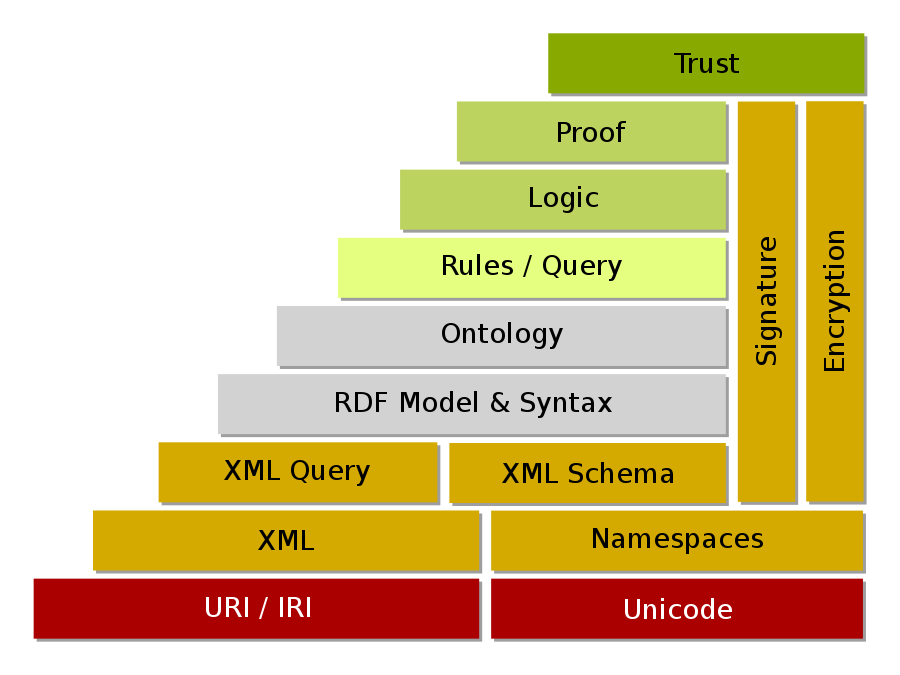
\includegraphics[width=0.7\textwidth]{images/semanticweblayers.png}
\caption{Livelli del web semantico \cite{semanticWebImage}}
\label{livelliWebSemantico}
\end{figure}

In Figura \ref{livelliWebSemantico} vi è una schematizzazione di questi livelli. 
Alla base, in rosso, troviamo il concetto di URI (Uniform resource identifier), ovvero un insieme di identificatori che rendono univoci i riferimenti, com'è spesso necessario nel momento in cui si scrive un testo.
A salire, in arancione, incontriamo la tecnologia XML \cite{xmlBook} (eXtensible Markup Language), linguaggio di markup che permette di creare tag personalizzati per descrivere una risorsa: si è così in grado di conferire una struttura arbitraria ai propri dati, pur senza dare informazioni su cosa questa struttura stia effettivamente a significare.
Il significato è demandato a RDF \cite{rdfBook} (in grigio in figura), standard proposto dal W3C; si tratta di un set di linguaggi basato su sintassi XML, principalmente utilizzato per fare delle asserzioni descrittive di un contenuto. RDF utilizza delle triple soggetto-verbo-oggetto, ad esempio ``Apprendimento di insiemi fuzzy nell'ambito del web semantico" (soggetto) ha come autore (predicato) Alessia Cecere (oggetto): questa particolare struttura risulta essere adatta a descrivere la maggior parte dei dati che devono essere elaborati da macchine.
I tre componenti di una tripla sono spesso rappresentati da URI, in modo da indicare elementi specifici ed evitare l'ambiguità tra termini che è tipica del linguaggio naturale.
Il passo successivo è dato dalla ontologie o OWL (Web ontology language) \cite{owlBook}, che permettono di superare la specificità dei riferimenti (ad esempio diversi modi di esprimere lo stesso concetto), tramite una tassonomia e un insieme di regole di inferenza. La tassonomia descrive classi di oggetti e le relazioni che queste classi hanno tra loro (ad esempio, ``sedia è una sottoclasse di mobile"), mentre le regole di inferenza permettono di stabilire vincoli ulteriori relativi alla realtà di riferimento: ad esempio, se un prefisso è associato a una città, e un indirizzo utilizza quel prefisso, allora anche l'indirizzo ha associato il prefisso di quella città \cite{semanticWebPaper}. 
L'utilizzo delle ontologie permette di salire al livello successivo, ovvero recuperare documenti esprimendo query complesse, che tengano conto non solo degli oggetti del discorso coinvolti ma anche del legame tra essi.
Si tratta del primo passo verso lo strato verde, ovvero il livello logico, non ancora sviluppato e oggetto di speculazione teorica. A questo livello l'obiettivo è realizzare sistemi composti da formulazioni di concetti logici e rendere i computer in grado di ragionare per inferenza su tali principi, attraverso lo scambio di informazioni tra un insieme di processori di informazioni. Naturalmente, in questo contesto dovrà essere garantito un grado di fiducia nelle informazioni incontrate, attraverso l'uso trasversale (arancione e verticale in figura) di crittografia e firma digitale: questa attesterà che un determinato utente ritiene veritiero un documento o un'istruzione, dando alle macchine dei parametri per stabilire in cosa e quanto credere.
Lo sviluppo di questi concetti porterà nel suo complesso alla realizzazione del \emph{Web of trust}: ogni utente avrà un insieme di utenti nei quali ha fiducia, che ne avranno a loro volta altri, a costruire una rete.

\section{Applicazione alla ricerca di assiomi in un insieme di formule}
\label{ontologyLearning}

L'ontology learning è un ambito di ricerca che punta alla generazione automatica di ontologie, a partire da un testo o un'ontologia preesistente (tipicamente espressa in OWL), insieme alla sua istanza (espressa in RDF). Sono stati studiati diversi metodi per ricavare dei pattern da questi input, e tutti si basano fortemente sul calcolo dello score di candidati assiomi, ovvero sull'identificazione del valore di verità delle formule di un insieme considerato, allo scopo di ricavarne degli assiomi.
Negli ultimi anni sono stati proposti diversi approcci alla risoluzione del problema, che utilizzano principalmente euristiche 
fondate su inferenza statistica.
Un'euristica basata sulla teoria della possibilità e sulla falsificazione nel contesto della semantica del mondo aperto viene proposta in \cite{possibilitypaper} e riassunta in \cite{sacpaper}.
Sintentizzando ulteriormente, immaginiamo di avere un candidato assioma $\phi$ che esprime una possibile relazione tra due elementi del dominio, e di dover valutare la sua credibilità sulla base di un dataset a disposizione $\Gamma$.
L'assioma $\phi$  verrà definito come l'insieme finito di affermazioni $\psi$  che ne sono conseguenza: perciò, se  $\Gamma \models\footnote{Il simbolo $\models$ esprime la relazione di conseguenza logica. In questo caso indica che, se tutte le proposizioni contenute nel dataset $\Gamma$ sono vere, allora ne deve conseguire che anche $\psi$ è vera.} \psi$ allora $\psi$ è una conferma di $\phi$, se $\Gamma \models \neg \psi$ allora $\psi$ è un controesempio di $\phi$, mentre se 
$\Gamma \not\models \psi$ e $\Gamma \not\models \neg \psi$ non si tratta né di un controesempio né di una conferma.
Inseriamo nel quadro la teoria della possibilità, ovvero quella teoria matematica per cui a ogni evento si associa un grado di possibilità tra 0 (impossibile) e 1 (completamente possibile, normale)\cite{DUBOIS200647}: avendo a disposizione una distribuzione di possibilità $\pi$, induciamo una misura di possibilità $\Pi$ per ogni evento. 
Indichiamo con $u_\phi$ la cardinalità degli $\psi$, con  $u_{\phi}^+$ la cardinalità delle conferme di $\phi$ e con $u_{\phi}^-$ la cardinalità dei controesempi di $\phi$; allora, se $u_\phi > 0,$  

\[ \Pi(\phi) = 1 - \sqrt{1 - \frac{u_\phi - u_{\phi}^-}{u_\phi}},\]
mentre se $u_\phi > 0,$ allora $\Pi(\phi) = 1$.
Il problema di questa tecnica è che, a meno di alcuni trucchi di implementazione, è impossibile da applicare nella pratica, a causa dell'eccessivo costo computazionale.

L'alternativa considerata per il lavoro che si andrà a documentare, esposta in \cite{sacpaper}, è quella di allenare un modello surrogato tramite un algoritmo di machine learning; l'allenamento viene fatto in modo induttivo a partire da un insieme di possibili assiomi e delle loro negazioni, etichettati con i rispettivi valori di possibilità precedentemente calcolati. L'obiettivo è rendere l'algoritmo in grado di ricavare valori di possibilità per nuovi candidati assiomi.


Il metodo è promettente perché il grande costo computazionale viene concentrato nella fase iniziale (il calcolo dei valori di possibilità ha richiesto poco meno di 290 giorni di tempo di CPU su una macchina piuttosto potente \cite{sacpaper}) e molto mitigato in quelle successive: una volta calcolati i valori di possibilità per le formule con cui allenare l'algoritmo ed effettuato il training, l'inferenza per i nuovi candidati assiomi sarà pressoché immediata.

L'algoritmo utilizzato, descritto nel Paragrafo \ref{algorithmParagraph}, si basa sull'inferenza di una funzione di appartenenza a un insieme fuzzy: l'insieme fuzzy è la classe degli assiomi, mentre il valore di possibilità con cui le formule sono inizialmente etichettate rappresenta il grado di appartenenza al suddetto insieme.
Il problema risulta adatto a essere modellato in senso fuzzy perché l'appartenenza alla categoria degli assiomi non è booleana: l'obiettivo non è suddividere le formule in categorie binarie di vero o falso, ma assegnare a ognuna di esse un certo valore di possibilità, grado di confidenza nel contesto incerto della modellazione della conoscenza. In questo senso, la confidenza nel candidato assioma sarà tanto più grande quanto il grado di appartenenza all'insieme fuzzy degli assiomi.

\chapter{Risoluzione del problema}
\section{L'algoritmo di apprendimento}\label{algorithmParagraph}
Per affrontare il problema sopra descritto, si è utilizzata una variante dell'algoritmo di support vector clustering, descritta in \cite{svpaper}.

Dati un campione  \{$x_1$, \dots , $x_n$\} di elementi appartenenti a un dominio $X$ e i rispettivi gradi di appartenenza  \{$\mu_1$, \dots , $\mu_n$\}  a un fuzzy set sconosciuto $A$, obiettivo dell'algoritmo è indurre un'approssimazione del fuzzy set $A$,  inferendo la sua funzione di appartenenza $\mu_A$. Per spiegare la tecnica, immaginiamo di dover trovare una sfera di raggio $R$  e centro $a$  che contenga i punti con membership elevata, in modo che il loro  grado di membership dipenda dalla distanza dal centro $a$.
Un primo modo di formulare il problema sarebbe, ignorando i valori di membership, la seguente ottimizzazione vincolata:
\[ \min R^2 + C\sum_{i} \xi_{i}\]
\[s.t.\]
\[||x_i - a||^2  \leq R^2 + \xi_{i} \; \forall i = 1, \dots, n,\]
\[ \xi_{i}\ \geq 0 \; \forall i = 1, \dots, n.\]
Il problema diventa dunque trovare la sfera di raggio minimo, al variare di $R^2$ e $a$, che raccolga la maggior parte dei punti rappresentanti gli elementi del campione.  
Le $\xi_i$ corrispondono a variabili di slack, che vengono aggiunte per rilassare i vincoli ove necessario, rendendoli ridondanti e permettendo che vengano rispettati, per alcune istanze, nonostante queste non si trovino all'interno della sfera. Per ridurre il numero di punti all'esterno della sfera, minimizziamo la somma delle $\xi_i$ all'interno della funzione obiettivo, moltiplicandola per un valore $C$, che funge da bilanciamento tra il rilassamento precedentemente descritto e il rispetto del vincolo, identificando se sia più importante mantenere vincoli stringenti o mappare tutti i punti nella sfera.
In realtà, l'obiettivo è che la distanza dal centro della sfera rappresenti un grado di appartenenza all'insieme fuzzy, e dunque andiamo a inserire le $\mu_i$ nella formulazione, che diventa:

\[\min R^2 + C\sum_{i} (\xi_{i} + \tau_{i})\]
\[s.t.\]
\[ \mu_i||x_i - a||^2  \leq \mu_i R^2 + \xi_{i} \; \forall i = 1, \dots, n,\]
\[ (1 - \mu_i)||x_i - a||^2  \geq \mu_i R^2 - \tau_{i}  \; \forall i = 1, \dots, n,\]
\[ \xi_{i}\ \geq 0, \tau_{i}\ \geq 0  \; \forall i = 1, \dots, n.\]

La formulazione cattura in parte l'insieme fuzzy, infatti:
\begin{itemize}
  \item Se  $\mu_i$ = 1, il secondo vincolo diventa ridondante, e si torna alla formulazione iniziale, nella quale si chiede di trovare il centro  e il raggio della sfera più piccola che contiene tutti i punti con membership 1;
  \item Se   $\mu_i$ = 0, è il primo vincolo a diventare ridondante, e il vincolo modula la non appartenenza alla sfera;		
  \item Se   $\mu_i$ = $\frac{1}{2}$, moltiplicando entrambi i vincoli per 2 si ottiene:
\[ ||x_i - a||^2  \leq R^2 + 2\xi_{i} \; \forall i = 1, \dots, n,\]
\[ ||x_i - a||^2  \geq R^2 - 2\tau_{i}\; \forall i = 1, \dots, n.\]
\end{itemize}

Dal momento che entrambe le variabili di slack devono essere il più possibile vicine e zero, questo sta a significare che per la membership  $\frac{1}{2}$ i punti tendono a stare esattamente sulla superficie della sfera. Dunque, risolvendo il problema di ottimizzazione, troviamo una prima approssimazione dell'insieme fuzzy, in termini di una sfera che conterrà i punti con membership elevata ed escluderà quelli con membership bassa, la cui frontiera identificherà il luogo dei punti con incertezza massima (con membership  $\frac{1}{2}$). Rimane il problema di modellazione delle membership intermedie, che si affronterà in seguito.
Ottenuta quest'ultima formulazione del problema di ottimizzazione, si risolve il corrispondente problema duale, attraverso il metodo di Wolfe. Per farlo, costruiamo la funzione lagrangiana, sottraendo all'obiettivo i vincoli, moltiplicati per altrettante variabili:

\[ L = R^2 + C\sum_{i}(\xi_i + \tau_i) - \sum_{i}\alpha_i(\mu_i \cdot R^2 + \xi_i - ||x_i - a||^2) +\] 
\[- \sum_{i}\beta_i[(1- \mu_i)||x_i - a||^2 - (1 - \mu_i)R^2 + \tau_i] -  \sum_{i}\gamma_i\xi_i - \sum_{i}\delta_i\tau_i.\]

Tale metodo richiede che tutte le derivate parziali della lagrangiana rispetto alle variabili del problema originale siano poste uguali a zero. Le suddette derivate assumono la seguente forma:
\[ \frac{\partial L}{\partial R^2} = 1- \sum_{i}\alpha_i\mu_i + \sum_{i}\beta_i(1 - \mu_i),\]
\[ \frac{\partial L}{\partial \xi_k} = C - 	\alpha_k - \gamma_k  \; \forall k = 1, \dots, n,\]
\[ \frac{\partial L}{\partial \tau_k} = C - \beta_k - \delta_k  \; \forall k = 1, \dots, n.\]

Sostituendo il pattern $\sum_{i}\alpha_i\mu_i - \beta_i(1-\mu_i)$ con $\epsilon_i$ e imponendo che derivata parziale rispetto a $R^2$ si annulli, otteniamo $\sum_{i}\epsilon_i = 1$.
Calcoliamo la derivata parziale della lagrangiana rispetto alla variabile originale $a$:

\[ \frac{\partial L}{\partial a} = \sum_{i}||x_i - a||^2\epsilon_i.\]

Imponendo che questa sia uguale a zero e tenendo conto del vincolo sulla sommatoria delle $\epsilon_i$ appena ricavato,  arriviamo all'equazione  $\sum_{i}x_i\epsilon_i = a$. Dunque, nel momento in cui si trovano le variabili ottimali $\epsilon_i$, si sa di riuscire a identificare anche il centro della sfera cercata.
Il problema duale, da massimizzare, è dunque:

\[ \max \sum_{i}\epsilon_ix_i\cdot x_i - \sum_{i,j}\epsilon_i\epsilon_jx_i\cdot x_j\]
\[s.t.\]
\[\sum_i\epsilon_i = 1.\]

Una volta risolto il problema e ottenute le $\epsilon_i^*$ ottimali, a partire da un qualunque elemento $x$ del dominio si può calcolare il valore:

\[ R^2(x) = x \cdot x - \sum_{i}\epsilon_i^*x_i \cdot x + \sum_{i,j}\epsilon_i^*\epsilon_j^*x_i \cdot x_j.\]

Si può dimostrare che questa quantità è esattamente uguale al quadrato della distanza tra $a^*$ (valore ottimale del centro) e $x$ fornito. Inoltre,  se si prende un $i$ tale che $0 < \alpha_{i}\ < C$ o $0 < \beta_{i}\ < C$,  allora $R^2(x_i) = R^*$, quadrato del raggio ottimale della sfera.
Perciò, dato un punto, è possibile stimare il suo grado di appartenenza alla sfera: se $R^2(x_i) > R^*$ ha membership $>\frac{1}{2}$, se $R^2(x_i)$ = $R^*$ la membership è  $\frac{1}{2}$, se $R^2(x_i)  < R^*$ la membership è  $< \frac{1}{2}$.
A questo punto, per ottenere un'approssimazione che rifletta anche le membership intermedie, è necessario stabilire una famiglia per la funzione di appartenenza che vogliamo inferire, ed eseguire una regressione all'interno di questa famiglia. Nel Paragrafo \ref{FuzzifierSection} vi è una descrizione delle famiglie di funzioni che sono state utilizzate allo scopo.

In realtà, l'ipotesi di racchiudere la maggior parte dei punti all'interno di una sfera è eccessivamente restrittiva: si rende pertanto necessario introdurre una trasformazione  $\Phi$, che mappi in modo non lineare tali punti in uno spazio di dimensione più elevata rispetto al dominio considerato; in questo spazio cercheremo la sfera che includa la maggior parte delle immagini.
La trasformazione $\Phi$ deve essere non lineare, in modo che la nuova sfera corrisponda, nello spazio originale, a un insieme che meglio si possa adattare ai dati. Definiamo kernel la funzione che accetta due argomenti e calcola il prodotto scalare delle loro immagini attraverso $\Phi$: questa si può calcolare anche non conoscendo la trasformazione specifica, ma sapendo a quale famiglia appartiene. Ad esempio, nel caso sia una funzione polinomiale di grado al massimo $p$, $k(x_i, x_j) = \Phi(x_i)\cdot \Phi(x_j) = (1 + x_i \cdot x_j)^p$.
Di conseguenza, la formulazione finale della funzione obiettivo diventa

\[ \max \sum_{i}\epsilon_i\Phi(x_i) \cdot \Phi(x_j) - \sum_{i,j}\epsilon_i\epsilon_j\Phi(x_i) \cdot \Phi(x_j),\]

mentre il calcolo di $R^2(x)$ viene così modificato:

\[ R^2(x) = \Phi(x) \cdot \Phi(x) - \sum_{i}\epsilon_i^*\Phi(x_i) \cdot x + \sum_{i,j}\epsilon_i^*\epsilon_j^*\Phi(x_i)\cdot \Phi(x_j).\]

Nel Paragrafo \ref{kernelSection} sono elencati e descritti i diversi kernel utilizzati durante gli esperimenti.

\subsection{Utilizzo della libreria mulearn}\label{FuzzifierSection}

Per eseguire gli esperimenti, è stata utilizzata la libreria mulearn \cite{mulearn}.
Come si può leggere dalla documentazione, al suo interno vi è una classe FuzzyInductor, che raccoglie la funzionalità fondamentale del processo di apprendimento: una volta allenato (attraverso l'operazione fit) su una serie di esempi, il FuzzyInductor è in grado, ricevendo un vettore di valori, di inferire una funzione di appartenenza all'insieme fuzzy, e quindi di restituire, tramite la funzione predict, un grado di appartenenza per ogni vettore dato.
Per la costruzione del FuzzyInductor devono essere specificati una serie di parametri; il primo dei quali è \texttt{c} (l'equivalente di $C$ dei paragrafi precedenti), che fa da tradeoff tra la grandezza della sfera di appartenenza e il rispetto dei vincoli imposti. 

Ulteriore parametro è il fuzzifier, ovvero la funzione che riceve come argomento la distanza tra l'immagine di un vettore $x$ e il centro della sfera (indicata con $R^2(x)$ nel paragrafo precedente), restituendo un'approssimazione del grado di appartenenza di $x$ al fuzzy set. Esistono diversi tipi di fuzzificatori, più o meno complessi a seconda delle esigenze del problema.
\begin{itemize}
\item \emph{Crisp Fuzzifier} (grafico esemplificativo in Figura \ref{crispFuzzifierGraph}): corrisponde a un insieme nel senso classico del termine, che ha valore 1 se l'elemento appartiene all'insieme, 0 se non vi appartiene;

\begin{minipage}{\linewidth}
	\centering
      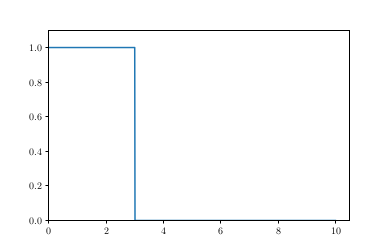
\includegraphics[width=0.8\linewidth]{images/crispFuzzifier.png}
	\captionof{figure}{Grafico esemplificativo di un crisp fuzzifier}
	\label{crispFuzzifierGraph}
\end{minipage}

\item \emph{Linear Fuzzifier}(grafico esemplificativo in Figura \ref{linearFuzzifierGraph}): corrisponde a un fuzzy set la cui membership decresce linearmente da 1 a 0;


\begin{minipage}{\linewidth}
	\centering
      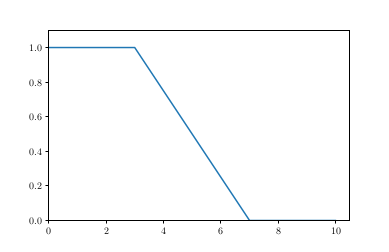
\includegraphics[width=0.8\linewidth]{images/linearFuzzifier.png}
	\captionof{figure}{Grafico esemplificativo di un linear fuzzifier}
	\label{linearFuzzifierGraph}
\end{minipage}

\item \emph{Exponential Fuzzifier}(grafico esemplificativo in Figura \ref{exponentialFuzzifierGraph}): corrisponde a un fuzzy set la cui  membership diminuisce da 1 a 0 in maniera esponenziale; la funzione che trasforma la distanza $r$ dal centro della sfera in un grado di appartenenza vale 1 se $r \leq r_1$, dove $r_1$ è il valore soglia, $e(r)$ altrimenti (dove $e$ è una funzione esponenziale che decresce da 0 a 1). Il parametro $\alpha$ indica il decadimento esponenziale fissato;

\begin{minipage}{\linewidth}
	\centering
       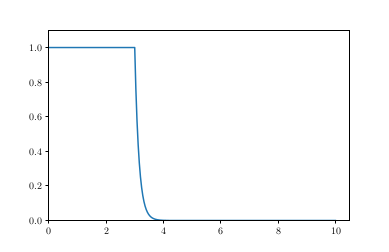
\includegraphics[width=0.8\linewidth]{images/exponentialFuzzifier.png}
	 \captionof{figure}{Grafico esemplificativo di un exponential fuzzifier con $\alpha$ = 0.001}
	 \label{exponentialFuzzifierGraph}
\end{minipage}

\begin{minipage}{\linewidth}
	\centering
       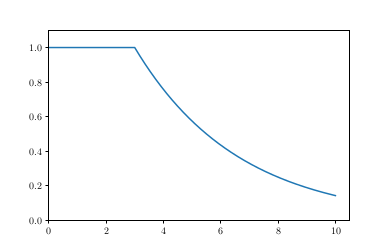
\includegraphics[width=0.8\linewidth]{images/exponentialFuzzifier2.png}
	 \captionof{figure}{Grafico esemplificativo di un exponential fuzzifier con $\alpha$  = 0.5}
\end{minipage}
\end{itemize}

Per tutti i fuzzificatori fin ora descritti è possibile fissare il parametro \texttt{profile} a \texttt{fixed} o \texttt{infer}: il primo esegue l'adattamento dei dati alla funzione di appartenenza basandosi su valori standard prefissati, mentre il secondo metodo modifica le soglie di riferimento a partire dai dati del campione. I fuzzificatori seguenti, invece, basandosi sui quantili, sono sempre adattati al campione specifico su cui vengono utilizzati.

\begin{itemize}
\item \emph{Quantile Constant Piecewise Fuzzifier}(grafico esemplificativo in Figura \ref{quantileConstantFuzzifierGraph}):  corrisponde a un fuzzy set che ha una funzione di membership costante a tratti, per la quale gli step sono definiti in base ai quartili delle distanze al quadrato tra le immagini dei punti e il centro della sfera inferita; 

\begin{minipage}{\linewidth}
	\centering
       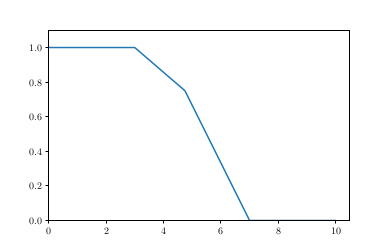
\includegraphics[width=0.8\linewidth]{images/quantileConstantPiecewiseFuzzifier.png}
	 \captionof{figure}{Grafico esemplificativo di un quantile constant piecewise fuzzifier}
	\label{quantileConstantFuzzifierGraph}
\end{minipage}

\item \emph{Quantile Linear Piecewise Fuzzifier}(grafico esemplificativo in Figura \ref{quantileLinearConstantFuzzifierGraph}):  corrisponde a un fuzzy set che ha una funzione di membership lineare a tratti, per la quale gli step sono definiti in base ai quartili delle distanze al quadrato tra le immagini dei punti e il centro della sfera inferita.

\begin{minipage}{\linewidth}
	\centering
       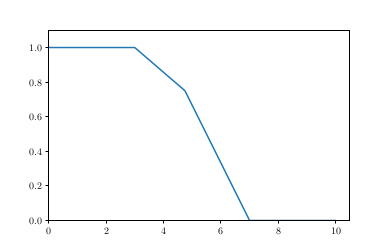
\includegraphics[width=0.8\linewidth]{images/quantileLinearPiecewiseFuzzifier.png}
	 \captionof{figure}{Grafico esemplificativo di un quantile linear piecewise fuzzifier}
	\label{quantileLinearConstantFuzzifierGraph}
\end{minipage}

\end{itemize}

Nella costruzione del FuzzyInductor si può optare per due tipi diversi di solver che risolvano il problema di ottimizzazione: il solver basato su Gurobi e quello basato su TensorFlow. 

Gurobi\cite{gurobi} è un solutore commerciale di ottimizzazione sviluppato nel 2008. Risolve problemi di programmazione lineare (LP), quadratica (QP), quadratica con vincoli (CQP), programmazione lineare intera mista (MILP), programmazione intera quadratica mista (MIQP) e programmazione intera quadratica con vincoli (MIQCP).

TensorFlow \cite{tensorFlow} è una piattaforma end-to-end open source per il machine learning. Viene utilizzata in ambiti di produzione e di ricerca scientifica, principalmente allo scopo di realizzare algoritmi per compiti percettivi e di comprensione del linguaggio. Viene tipicamente utilizzato per allenare modelli di reti neurali profonde, ma, dal momento che il loro allenamento richiede l'ottimizzazione di una funzione (funzione di perdita), è possibile utilizzarlo per risolvere problemi generici di ottimizzazione, come il quello descritto nel Paragrafo \ref{algorithmParagraph}.

\section{Il Kernel}\label{kernelSection}
Il parametro kernel (equivalente della funzione $k$ dei paragrafi precedenti) della classe FuzzyInductor definisce quale sarà la funzione attraverso cui i valori verranno mappati nello spazio a più dimensioni.
La libreria mulearn implementa i seguenti kernel:

\begin{itemize}
\item \emph{kernel lineare}: il valore $k(x_1,x_2)$ equivale al prodotto $x_1\cdot x_2$, ovvero  $\sum_{i=1}^N(x_1)_i\cdot(x_2)_i$, dove $N$ è la dimensione dei vettori $x_1$ e $x_2$;
\item \emph{kernel polinomiale}: il valore $k(x_1,x_2)$ equivale a $(x_1\cdot x_2 + 1)^d$, dove $d$ è il grado polinomiale del kernel;
\item \emph{kernel polinomiale omogeneo}:  il valore  $k(x_1,x_2)$ equivale a $(x_1\cdot x_2)^d$;
\item \emph{kernel Gaussiano}:   il valore  $k(x_1,x_2)$ equivale a $e^{-\frac{||x_1 - x_2||^2}{2 \sigma^2}}$, dove $\sigma$ è la deviazione standard del kernel;
\item \emph{kernel iperbolico}:   il valore $k(x_1,x_2)$  equivale a $\tanh(\alpha x_1 \cdot x_2 + \beta)$, dove $\alpha$ è la scala e $\beta$ l'offset.
\end{itemize}

La maggior parte dei kernel qui descritti richiedono di essere inizializzati con opportuni iper-parametri: nel Capitolo \ref{capitoloEsperimenti} è stato esposto il procedimento di model selection effettuato su di essi.

\subsection{Kernel precomputato}
\label{jaccardSection}
Per ottimizzare i tempi di computazione (i punti da mappare, nel caso di un insieme di formule, non corrispondono a valori numerici i cui valori del kernel sono semplici da calcolare) si è utilizzato un kernel precomputato: il valore di  $k(x_1,x_2)$ non viene calcolato sul momento, ma prelevato da una matrice precalcolata con i valori del kernel per ogni coppia di candidati assiomi, detta \emph{matrice di Gram}.
In generale, il valore restituito da un kernel è interpretabile come una misura della similarità (sim) tra i suoi argomenti: per calcolarlo tra due formule si è dunque fatto riferimento a un criterio ispirato alla similarità di Jaccard, descritto in \cite{sacpaper}.
Per tutte le coppie di assiomi $\phi$ e $\psi$, la definizione di similarità deve rispettare le seguenti proprietà:
\begin{itemize}
\item $0 \leq \mathrm{sim(\psi, \phi)} \leq 1$, si sta infatti operando in un ambito possibilistico, nel quale a ogni assioma viene associato un grado di possibilità compreso tra 0 e 1;
\item $\mathrm{sim(\psi, \phi)} = 1$ sse $\psi \equiv \phi $;
\item $\mathrm{sim(\psi, \phi)} = \mathrm{sim(\phi,\psi)}$.
\end{itemize}
Se si riuscisse a definire una funzione $\mathrm{Impl(\phi,\psi)}$, a indicare la relazione di implicazione materiale, allora si potrebbe dire

\[  \mathrm{sim(\psi, \phi)} = \min \{\mathrm{Impl(\phi,\psi)}, \mathrm{Impl(\psi,\phi)}\}, \]

dove il minimo traduce la congiunzione delle due condizioni logiche.
Per definire l'implicazione, ci si può avvalere della sua definizione classica, ovvero $\mathrm{Impl(\psi,\phi)} = 1$ se $\models \lnot \phi \lor \psi$, 0 altrimenti.


Si può restringere il campo agli assiomi di inclusione di cui ci si è occupati nello specifico, ovvero formule del tipo Subclass(B,C), o 	$B \sqsubseteq C$ in forma più compatta, e le loro negazioni \emph{ $\lnot \mathrm{Subclass(B,C)}$} ({$ B \not\sqsubseteq C$}).
Avendo a disposizione un insieme di assiomi, si può dire che un individuo della base di conoscenza $a$ conferma $B \sqsubseteq C$ (e contraddice  {$ B \not\sqsubseteq C$}) se vale $B(a) \land C(a)$, $a$ contraddice  $B \sqsubseteq C$ (e conferma {$ B \not\sqsubseteq C$}) se vale $B(a) \land \lnot C(a)$.
Dunque, sfruttando la definizione precedentemente data di implicazione materiale, si può affermare:

\[Impl(A \sqsubseteq B, C \sqsubseteq D) = \frac{\parallel \{ a: (A(a) \land \lnot B(a)) \lor (C(a) \land D(a)) \} \parallel}{\parallel \{ a: (A(a) \lor C(a))\} \parallel}. \]

Se si definisce

\[ [C] = \{a : C(a) \},\]

allora si può scrivere la formula precedente come:

\[ \frac{\parallel [A] \cup [\overline{B}] \cup [C] \cap [D] \parallel}{\parallel [A] \cup [C] \parallel}.\]

Avendo precedentemente definito l'operatore di similarità tra due assiomi in relazione al minimo tra le due implicazioni, risulta:

\[ sim(A \sqsubseteq B, C  \sqsubseteq D) = min\{Impl(A \sqsubseteq B, C\sqsubseteq D), Impl( C\sqsubseteq D, A \sqsubseteq B)\} \]
\[ = min\bigg\{\frac{\parallel [A] \cap [\overline{B}] \cup [C] \cap [D] \parallel}{\parallel [A] \cup [C] \parallel}, \frac{\parallel [C] \cup [\overline{D}] \cup [C] \cap [D] \parallel}{\parallel [A] \cup [C] \parallel}\bigg\}.\]
\[ = \frac{min\{\parallel [A] \cap [\overline{B}] \cup [C] \cap [D] \parallel, \parallel [C] \cup [\overline{D}] \cup [C] \cap [D] \parallel\}}{\parallel [A] \cup [C] \parallel}.\]

Nella pratica, per calcolare i valori del kernel precomputato si è utilizzata una versione semplificata della formula precedente, ovvero:

\[sim(A \sqsubseteq B, C  \sqsubseteq D) = \frac{\parallel [A] \cap [B] \cup [C] \cap [D] \parallel}{\parallel [A] \cup [C] \parallel}. \]


\subsection{Kernel alternativi}
Nel corso degli esperimenti sono state utilizzate altre definizioni di similarità, diverse da quella di Jaccard, descritte in \cite{drtpaper}.
\subsubsection{Length-based similarity}
\label{lengthSection}
Una prima forma ingenua di similarità utilizzata è quella basata sulla lunghezza degli assiomi.
Si definisce dunque
\[ s_{len}(\phi_1, \phi_2) = 1 - \frac{|\# \phi_1 - \# \phi_2|}{max\{\#\phi_1, \#\phi_2\}},\]
ovvero il valore assoluto della differenza tra le due lunghezze, normalizzato.
Tale formulazione nasconde una problematica: quando un assioma è il negato dell'altro la funzione restituisce un valore di similarità alto. Occore, pertanto, introdurre un'ulteriore casistica: se i segni dei due assiomi sono diversi, la funzione di similarità vale $1 - s_{len}(\phi_1,\phi_2)$. Al Paragrafo \ref{esperimentiLength} si trova la descrizione degli esperimenti effettuati con questa misura di similarità.

\subsubsection{Hamming similarity}
\label{hammingSection}
Altro modo di definire la similarità tra due assiomi è la distanza di Hamming, ovvero la distanza tra le rappresentazioni testuali delle due formule, intesa come il numero di caratteri diversi tra una e l'altra, trascurando i caratteri extra della stringa più lunga.
Definendo $H$ la distanza di Hamming, si fa la stessa distinzione descritta precedentemente per gli assiomi di segno opposto:  $ \mathrm{sim_{H}}(\phi_1, \phi_2) = H(\mathrm{abs}(\phi_1),\mathrm{abs}(\phi_2))$ se i segni delle due formule sono opposti, $1 - H(\phi_1, \phi_2)$ altrimenti. Gli esperimenti relativi sono descritti al Paragrafo \ref{esperimentiHamming}.

\subsubsection{Levenshtein similarity}
\label{levenshteinSection}
L'ultima funzione di similarità utilizzata è la distanza di Levenshtein tra due stringhe, ovvero il numero più piccolo di operazioni atomiche che vanno fatte per trasformare una nell'altra. Chiamando questa funzione \emph{Lev}, $sim_{edit}(\phi_1, \phi_2) = 1 - Lev(\phi_1,\phi_2)$ se i due segni sono diversi, $Lev(abs(\phi_1),abs(\phi_2))$ altrimenti. Questa forma di similarità è utilizzata negli esperimenti al Paragrafo  \ref{esperimentiLevenshtein}.


\chapter{Esperimenti}\label{capitoloEsperimenti}

\section{Model selection e model evaluation}
La model selection è il processo di scelta di un modello definitivo tra un insieme di candidati modelli di machine learning per un training set; può essere applicata sia tra modelli sia tra parametri di uno stesso modello.
La model evaluation è, invece, la valutazione delle performance di un modello esistente.

Effettuare model selection e model evaluation sugli stessi dati che vengono utilizzati per il training  è un errore metodologico \cite{scikit-learn} che rende difficile identificare una condizione di overfitting, nella quale l'algoritmo è in grado di associare molto bene etichette a individui del campione che ha già visto, semplicemente ripetendole, ma fallisce nell'identificare i valori associati a nuovi elementi su cui non è stato allenato; spesso l'overfitting si verifica quando il numero di parametri è eccessivo rispetto a quello di osservazioni, dunque il modello risulta troppo complesso e finisce per adattarsi ai dati del campione, imparandone anche il ``rumore" (o informazioni irrilevanti) \cite{IBMlearning}.
Per questo motivo gli elementi del dataset vengono divisi in in training, validation e test set, utilizzati rispettivamente per allenare, selezionare e valutare i modelli.
Si tratta di un procedimento che può essere applicato quando si ha a disposizione una quantità consistente di dati: in molte situazioni, tuttavia, le quantità di dati disponibili per training e test saranno limitate. Per costruire dei buoni modelli vorremmo usare gran parte dei dati disponibili per il training, ma allo stesso tempo la scarsità di dati di test ci porterebbe a una valutazione poco attendibile dei modelli stessi \cite{patternRecognitionML}.	
Per far fronte a questa problematica, si deve fare riferimento ad altre strategie.

\subsection{Metodi probabilistici}

Un metodo di risolvere il problema è ricorrere a un approccio probabilistico, nel quale la valutazione del modello avviene basandosi contemporaneamente sulla sua complessità e sulle sue performance in fase di allenamento.
Dal momento che l'errore in fase di training tende notoriamente a essere sottostimato, lo scoring delle performance viene penalizzato sulla base di quanto alto si suppone questo bias di ottimismo, mentre la complessità dipende tipicamente dal numero di gradi di libertà dei parametri del modello.

Esistono principalmente tre approcci, derivati da diversi ambiti di ricerca:
\begin{itemize}
	\item{Akaike information criterion (AIC), derivato dalla probabilità frequentista;}
	\item{bayesian information criterion (BIC), derivato dalla probabilità bayesiana;}
	\item{minimum description length (MDL), derivato dalla teoria dell'informazione.}
\end{itemize}

Tutti utilizzano la \emph{log-likelihood} tra modello e dati, dove per log-likelihood si intende una variazione della maximum likelihood estimation, nella quale l'obiettivo è massimizzare la probabilità condizionata di osservare il dato ($X$), data una distribuzione di probabilità e i suoi parametri $\theta$, ovvero $P(X, \theta)$. $X$ può essere vista come la distribuzione di probabilità congiunta di tutte le osservazioni del dominio del problema da 1 a $n$, dunque formalmente $P(x_1, x_2, x_3 \dots x_n, \theta)$: la probabilità congiunta si può calcolare come la moltiplicazione delle probabilità condizionate di osservare ogni elemento, dati i parametri della distribuzione. Dal momento che, però, moltiplicare tutte le piccole probabilità porterebbe a instabilità, si riformula il tutto come la somma dei logaritmi naturali delle probabilità condizionate, ovvero la log-likelihood estimation, definita come $\sum_{i=1}^n\log(P(x_i,\theta))$.
Una descrizione estensiva di tutti i metodi probabilistici va al di fuori degli scopi di questo elaborato; si riporta tuttavia come esempio il caso dell'AIC, definito come la minimizzazione di $-2/N \cdot LL + 2k/N$ \cite{probabilisticMethod}, dove $N$ è il numero di elementi del campione, $LL$ la log-likelihood del modello sul traning set e $k$ il numero di parametri del modello.

Il vantaggio di questi approcci sta nel fatto che non necessitano di isolare una porzione di dati di test: tutti i dati a disposizione possono essere utilizzati per il training. I metodi probabilistici, tuttavia, non permettono di utilizzare lo stesso criterio per valutare più modelli (i criteri di valutazione tendono ad essere specifici per ogni modello, proprio a causa della loro variabilità) e non considerano l'incertezza dei parametri: nella pratica, questi metodi tendono a favorire modelli troppo semplificati \cite{APM}.
\subsection{Metodi di sottocampionamento}

I metodi di ricampionamento stimano le performance di un modello tramite elementi fuori dal campione di training.
Il traning set viene suddiviso in sottoinsiemi di training e di test, sui quali viene rispettivamente allenato e valutato, e questa suddivisione avviene più volte, riportando come errore finale la media delle performance degli esperimenti effettuati con ogni suddivisione.
Tra i metodi di ricampionamento contiamo:

\begin{itemize}
\item{\emph{random train/test splits}}: fissate le percentuali di dati che devono essere inserite nei sottoinsiemi di training e test,  l'assegnamento di un'osservazione a un campione o all'altro avviene in maniera casuale (in alcuni casi è meglio effettuare una stratificazione, ovvero una suddivisione preliminare dei dati in categorie, dette strati, da cui poi si estraggono casualmente i campioni, in modo da mantenere il bilanciamento dei dati del dataset intero \cite{introStat});

\item{\emph{bootstrap}}: per ognuno dei sottoinsiemi di training e test, si sceglie una grandezza del campione $n$, dopodiché,  scelta casualmente $n$ volte un'osservazione dal dataset, questa viene aggiunta al campione (la stessa osservazione può così trovarsi in più sottoinsiemi contemporaneamente); 
\item{\emph{cross-validation}}: in quanto metodo utilizzato per effettuare la maggior parte degli esperimenti di cui si tratterà in questo elaborato, la sua forma di base ($k$-Fold cross-validation) viene trattata nella sezione seguente.
\end{itemize}

\subsubsection{$k$-Fold cross-validation}
\label{kFoldCrossValidationSection}
Nella $k$-Fold cross-validation, il training set viene suddiviso in $k$ sottoinsiemi approssimativamente della stessa grandezza: per ogni sottoinsieme il modello viene allenato su $k - 1$ sottoinsiemi del training set, mentre la valutazione avviene sulla porzione rimanente dei dati; l'errore finale è dato dalla media degli errori calcolati per ogni ripetizione del processo.
Tale metodo risulta essere un compromesso tra l'utilizzo di un unico split di train/test e la ricerca di tutti i modi possibili di suddividere i dati a disposizione tra train e test set di ampiezza prefissata; permette inoltre di utilizzare tutti i dati a disposizione per allenare l'algoritmo, valore aggiunto che risulta determinante in problemi per i quali il numero di elementi del campione risulta basso \cite{scikit-learn}. Una schematizzazione grafica di questa tecnica viene riportata in Figura \ref{scikitSchema}.

\begin{figure}[h]	
\centering
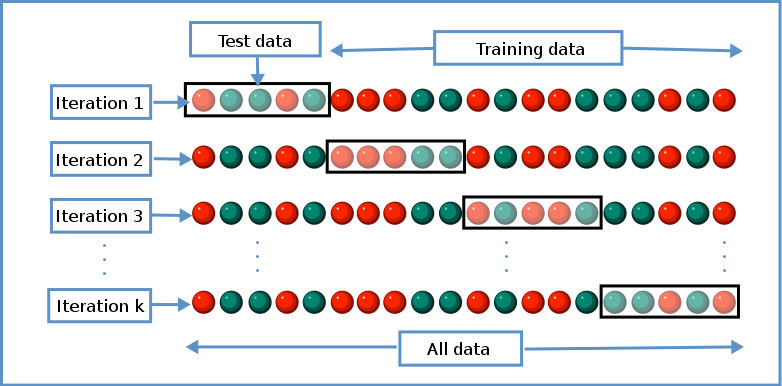
\includegraphics[width=0.9\textwidth]{images/782px-K-fold_cross_validation_EN.svg.png}
\caption{Schematizzazione della suddivisione in fold nella $k$-fold cross validation \cite{crossValidationImage}.}
\label{scikitSchema}
\end{figure}

\section{Riproduzione degli esperimenti originali}
Una delle prime attività svolte è stata quella di ripetere gli esperimenti originali descritti in \cite{sacpaper}, i cui valori medi di RMSE sono riportati nella Tabella \ref{table: risultatiVecchiEsperimenti}, per confrontarne i risultati al netto dell'utilizzo di una nuova libreria: quegli esperimenti, infatti, si basavano una versione vecchia del codice, che non era ancora stato organizzato sistematicamente come nella libreria mulearn \cite{mulearn}.

Sono stati considerati 722 candidati assiomi del tipo \emph{SubClassOf} con le loro negazioni, per un totale di 1444 formule;  tra ciascuna coppia è stata calcolata la similarità di Jaccard (introdotta al Paragrafo \ref{jaccardSection}) e inserita all'interno di una matrice di Gram $K$.
Il valore precalcolato di possibilità, il cui calcolo è descritto al Paragrafo \ref{ontologyLearning}, è stato utilizzato come etichetta per il grado di appartenenza di ogni formula all'insieme fuzzy degli assiomi.
Si è poi effettuata la model selection sugli iperparametri con cui inizializzare i componenti dell'algoritmo; le formule sono state permutate e divise in tre gruppi dedicati a training, model selection e model validation, contenenti rispettivamente l'80\% (1156 formule), il 10\% (144 formule) e il 10\% (144 formule) del campione originale (1444 formule).
La model selection è stata effettuata a questo stadio sull'iperparametro c, in termini di quale tra quelli testati (0.005, 0.007, 0.01, 0.03, 0.05, 0.07, 0.1, 0.3, 0.5, 0.7, 1, 10, 100) desse luogo all'RMSE minore nella previsione del grado di membership dell'assioma, dove RMSE sta a indicare lo scarto quadratico medio posto sotto radice, per riportarlo all'unità di misura dei dati.
Questo procedimento è stato ripetuto dieci volte per ogni fuzzificatore, concludendo per ciascuno di esso i valori minimi dell'RMSE sui valori di test, che vengono riportati nella Tabella \ref{table: risultatiNuoviEsperimenti}

\begin{table}[h!]
\centering 	
	\begin{tabular}{|l|l|} 
	 \hline
	  & RMSE test(+/- std) \\ [0.5ex] 
	 \hline
	 Crisp Fuzzifier & 0.41536 +/- 0.06\\ 
	 \hline
	 Quantile Constant Piecewise Fuzzifier & 0.33295 +/- 0.048\\
	 \hline
	 Quantile Linear Piecewise Fuzzifier & 0.30343 +/- 0.032\\
	 \hline
	 Linear Fuzzifier & 0.34012 +/- 0.054\\
	 \hline
	 Exponential Fuzzifier & 0.32827 +/- 0.04\\ [1ex] 
	 \hline
	\end{tabular}
	\caption{Valori minimi RMSE per fuzzificatore, esperimenti nuovi}
	\label{table: risultatiNuoviEsperimenti}
\end{table}

\begin{table}[h!]
\centering 	
	\begin{tabular}{|l|l|} 
	 \hline
	  & RMSE test(+/- std) \\ [0.5ex] 
	 \hline
	 Crisp Fuzzifier & 0.377 +/- 0.33\\ 
	 \hline
	 Quantile Constant Piecewise Fuzzifier & 0.314 +/- 0.179\\
	 \hline
	 Quantile Linear Piecewise Fuzzifier &  0.314 +/- 0.164\\
	 \hline
	 Linear Fuzzifier &  0.313 +/- 0.49 \\
	 \hline
	 Exponential Fuzzifier & 0.362+/- 0.321\\ [1ex] 
	 \hline
	\end{tabular}
	\caption{Valori minimi RMSE per fuzzificatore, esperimenti 2018}
	\label{table: risultatiVecchiEsperimenti}
\end{table}

Come si può notare confrontando le Tabelle \ref{table: risultatiNuoviEsperimenti} e \ref{table: risultatiVecchiEsperimenti}, i risultati ottenuti nei due esperimenti si discostano, anche se non eccessivamente.
Le maggiori differenze si riscontrano per il Crisp Fuzzifier e il Linear Fuzzifier; i risultati ottenuti mediante Exponential Fuzzifier sono solo parzialmente confrontabili poiché nel primo caso è stato utilizzato un fuzzificatore con decadimento esponenziale non fissato manualmente, mentre i risultati degli esperimenti del 2018 si riferiscono a un decadimento esponenziale di 0.001.
In generale, la deviazione standard dei nuovi esperimenti risulta essere di un ordine di grandezza inferiore, riflettendo risultati più stabili (intorno alla media) di quelli del 2018.
La Tabella \ref{table: confrontoIntervalli} riporta gli intervalli di errore, centrati sulla media e di semiampiezza deviazione standard, per gli esperimenti nuovi e vecchi.

\begin{table}[h!]
\centering 	
\small
	\begin{tabular}{|l|l|l|} 
	 \hline
	 Fuzzifier & Esperimenti nuovi & Esperimenti 2018\\ [0.5ex] 
	 \hline
	 Crisp & 0.35536 - 0.47536 & 0.047 - 0.707\\ 
	 \hline
	 Quantile Constant Piecewise & 0.28495 - 0.38095 & 0.135 - 0.493\\
	 \hline
	 Quantile Linear Piecewise & 0.27143 - 0.33 &  0.15 - 0.478\\
	 \hline
	 Linear & 0.28612 - 0.39412  &  -0,177 - 0.803 \\
	 \hline
	 Exponential  & 0.28827 - 0.36827 & 0.041 - 0.683\\ [1ex] 
	 \hline
	\end{tabular}
	\caption{Intervalli di RMSE per gli esperiementi vecchi e nuovi, centrati sull'RMSE medio e con semiampiezza deviazione standard}
	\label{table: confrontoIntervalli}
\end{table}

Gli intervalli d'errore di Crisp Fuzzifier e Linear Fuzzifier sono molto più elevati negli esperimenti vecchi che in quelli nuovi: ciò significa che gli esperimenti del 2018 riportano valori d'errore molto bassi all'estremo inferiore dell'intervallo e molto alti all'estremo superiore, mostrando una notevole instabilità.
 La situazione si ripete anche con gli altri fuzzificatori, sebbene con differenze meno nette.
Nei nuovi esperimenti il fuzzificatore con RMSE migliore risulta essere il Quantile Linear Piecewise Fuzzifier, che riporta il valore minimo più basso e anche l'ampiezza minore dell'intervallo, mentre negli esperimenti del 2018 il valore inferiore dell'intervallo d'errore del Quantile Constant Piecewise Fuzzifier è leggermente più basso, con intervalli di variazione comparabili.

\section{Esperimenti sul kernel}

Sono poi state effettuate model selection e model validation tramite $k$-Fold cross-validation (descritta al Paragrafo \ref{kFoldCrossValidationSection}) , con $k$ = 5, per ogni fuzzificatore.

La model selection è stata eseguita sul parametro \texttt{c}, scegliendo tra sette possibili valori in un range da -1 a 1, spaziati uniformemente su una scala logaritmica (dunque tra 0.1, 0.21544347, 0.46415888,  1,  2.15443469, 4.64158883 e 10).
Per ogni fuzzificatore, la model evaluation ha portato ai valori medi di RMSE in fase di test e in fase di train per i valori migliori di $c$, con le rispettive deviazioni standard.

Il procedimento è stato ripetuto utilizzando diversi kernel precomputati e ha portato ai risultati che verranno esposti nei paragrafi successivi.

\subsection{Esperimenti con Jaccard similarity}
Nella Tabella \ref{table:risultatiJaccard} sono riportati i  risultati ottenuti utilizzando come kernel la similarità di Jaccard definita nel Paragrafo \ref{jaccardSection}, precomputata e inserita all'interno di una matrice di Gram.

\begin{table}[h!]
\small
\centering 	
	\begin{tabular}{|c|c|c|}
	 \hline
	 Fuzzifier & RMSE test(+/- std) & RMSE train (+/- std)\\ [0.5ex] 
	 \hline
	 Crisp & 0.26974 +/ 0.27 & 0.21694 +/- 0.024 \\ 
	 \hline
	 Quantile Constant Piecewise & 0.11759 +/- 0.108 & 0.10881 +/- 0.02\\
	 \hline
	 Quantile Linear Piecewise & 0.1032 +/- 0.08 & 0.09935 +/- 0.014\\
	 \hline
	 Linear & 0.15256 +/- 0.172 & 0.13883 +/- 0.024\\
	 \hline
	 Exponential  & 0.13603 +/- 0.17 & 0.13391 +/- 0.02\\ [1ex] 
	 \hline
	\end{tabular}
\caption{Valori medi di RMSE in fase di test e train per ogni fuzzificatore, con la similarità di Jaccard come kernel.}
\label{table:risultatiJaccard}
\end{table}


\subsection{Esperimenti con Length-based similarity}
\label{esperimentiLength}
La Tabella \ref{table:risultatiLength} mostra i risultati ottenuti utilizzando come kernel la similarità basata su lunghezza definita al Paragrafo \ref{lengthSection}. L'ingenuità del metodo faceva supporre un generale peggioramento dei risultati rispetto alla similarità di Jaccard in Tabella \ref{table:risultatiJaccard}, che anzi si presupponeva più consistente di quello effettivamente riscontrato.

\begin{table}[h!]
\small
\centering 	
	\begin{tabular}{|c|c|c|} 
	 \hline
	 Fuzzifier & RMSE test(+/- std) & RMSE train (+/- std)\\ [0.5ex] 
	 \hline
	 Crisp & 0.38573 +/- 0.466 & 0.391 +/- 0.108 \\ 
	 \hline
	 Quantile Constant Piecewise & 0.31572 +/- 0.288 & 0.31 +/- 0.058\\
	 \hline
	 Quantile Linear Piecewise & 0.30646 +/- 0.252 & 0.3 +/- 0.052\\
	 \hline
	 Linear & 0.24792 +/- 0.092 & 0.225 +/- 0.014\\
	 \hline
	 Exponential & 0.24521 +/- 0.11 & 0.224 +/- 0.014\\ [1ex] 
	 \hline
	\end{tabular}
	\caption{Valori medi di RMSE in fase di test e train per ogni fuzzificatore, con la Length-similarity come kernel.}	
	\label{table:risultatiLength}
\end{table}

Una nuova classe kernel è stata implementata per essere utilizzata in modo da computare direttamente il valore di similarità basato su lunghezza dei due assiomi, senza passare per la creazione o il caricamento della matrice di Gram con i valori precalcolati.
Per velocità di computazione si è scelto di implementare solamente la prima versione della funzione, ignorando il problema del valore di similarità per assiomi opposti l'uno all'altro esposto nel Paragrafo \ref{lengthSection}.
Anche agendo in questo modo, il tempo di computazione è risultato accettabile eseguendo gli esperimenti su un massimo di 50 assiomi su 1444; si è scelto, pertanto, di utilizzare matrice e kernel precomputato anche per questa definizione di similarità. 

\subsection{Esperimenti con Hamming similarity}
\label{esperimentiHamming}
 Gli esperimenti con la Hamming similarity descritta al Paragrafo \ref{hammingSection} hanno invece condotto ai risultati riportati nella Tabella \ref{table:risultatiHamming}. I valori di RMSE e varianza risultano complessivamente peggiori rispetto alla similarità di Jaccard, e stranamente non molto migliori di quelli basati sulla lunghezza: anzi, utilizzando il CrispFuzzifier risultano essere perfino peggiori di questi ultimi.

\begin{table}[h!]
\small
\centering 	
	\begin{tabular}{|c|c|c|} 
	 \hline
	  Fuzzifier & RMSE test(+/- std) & RMSE train (+/- std)\\ [0.5ex] 
	 \hline
	 Crisp & 0.54868 +/- 0.418 & 0.713 +/- 0.118 \\ 
	 \hline
	 Quantile Constant Piecewise & 0.35935 +/- 0.198 & 0.448 +/- 0.064\\
	 \hline
	 Quantile Linear Piecewise & 0.35008 +/- 0.162 & 0.42 +/- 0.06\\
	 \hline
	 Linear &0.23933 +/- 0.11 & 0.191 +/- 0.066\\
	 \hline
	 Exponential & 0.22399 +/- 0.088 & 0.198 +/- 0.016\\ [1ex] 
	 \hline
	\end{tabular}
	\caption{Valori medi di RMSE in fase di test e train per ogni fuzzificatore, con la Hamming similarity come kernel.}
	\label{table:risultatiHamming}
\end{table}

Anche in questo caso, l'implementazione della classe \emph{HammingKernel} non ha portato ai risultati sperati, a causa dell'eccessivo costo computazionale di calcolare di volta in volta la distanza di Hamming per ognuno dei 1444 assiomi.

\subsection{Esperimenti con Levenshtein similarity}
\label{esperimentiLevenshtein}
 I valori dell'RMSE ottenuti tramite similarità di Levenshtein (Paragrafo \ref{levenshteinSection}) sono mostrati nella Tabella \ref{table:risultatiLevenshtein} e risultano valere le stesse considerazioni fatte per la distanza di Hamming.


\begin{table}[h!]
\small
\centering 	
	\begin{tabular}{|c|c|c|} 
	 \hline
	  Fuzzifier & RMSE test(+/- std) & RMSE train (+/- std)\\ [0.5ex] 
	 \hline
	 Crisp & 0.50254 +/- 0.388 & 0.73 +/- 0.076 \\ 
	 \hline
	 Quantile Constant Piecewise & 0.36324 +/- 0.122 & 0.439 +/- 0.058\\
	 \hline
	 Quantile Linear Piecewise & 0.35503 +/- 0.138	 & 0.412 +/- 0.05\\
	 \hline
	 Linear & 0.23958 +/- 0.094 & 0.201 +/- 0.068\\
	 \hline
	 Exponential & 0.23807 +/- 0.11 & 0.198 +/- 0.07\\ [1ex] 
	 \hline
	\end{tabular}
	\caption{Valori medi di RMSE in fase di test e train per ogni fuzzificatore, con la Levenshtein similarity come kernel.}
	\label{table:risultatiLevenshtein}
\end{table}

Come nei due casi precedenti, si è continuato a dover utilizzare una matrice di Gram precalcolata per definire i valori del kernel in un tempo accettabile.

\subsection{Il problema del raggio negativo}

Nel corso degli esperimenti, ci si è trovati di fronte a una problematica precedentemente inaspettata. 
Al momento del calcolo della distanza dei punti, nello spazio delle feature, dal centro dello spazio di riferimento, si è riscontrato che questi valori risultavano negativi. Questo non dovrebbe chiaramente avvenire per il valore di una distanza, e ha fatto sì che risultasse problematico considerare valido il valore di membership inferito dall'algoritmo per alcuni assiomi.

Il problema di definire perché ciò avvenga è ancora aperto, ma in prima istanza è stata fatta la seguente ipotesi: i valori del kernel all'interno della matrice di Gram sono stati precalcolati seguendo delle euristiche, che per definizione risultano intuitivamente corrette, ma non supportate da una dimostrazione formale. L'ipotesi è, dunque, che i valori precomputati della matrice di Gram non rappresentino effettivamente un kernel, non esistendo una dimostrazione del fatto che ne  rispettino le caratteristiche formali; perciò è possibile che, nel momento in cui si è andati a cercare di ritrovare delle proprietà matematiche che si riconoscevano immediate, queste non siano invece state riscontrate. 
Per cercare di comprendere meglio le ragioni che portavano al problema sopra descritto, sono stati condotti ulteriori esperimenti.

\subsubsection{Eliminazione di formule}
Contestualmente alla negatività del raggio, ci si è anche resi conto di un problema riguardante la matrice di Gram in sé: questa non era semidefinita positiva, requisito necessario per effettuare il processo di ottimizzazione. Teoricamente è possibile perturbare la diagonale della matrice al fine di renderla semidefinita positiva, ma l'aggiustamento necessario è risultato di un ordine di grandezza talmente elevato da far perdere di significato ai valori del kernel. Si è quindi supposto che il problema riguardasse la matrice, e, per convalidare l'ipotesi, si è pensato eliminare da quest'ultima alcune formule, allo scopo di capire se rimuovendole sarebbe cambiato anche l'aggiustamento. Inizialmente si è intrapresa una strada combinatoria, che consisteva nell'eliminare tutte le possibili formule una alla volta, successivamente tutte le coppie e a procedere fino a gruppi di dimensione più elevata; eliminando una formula alla volta non si sono riscontrati cambiamenti dell'aggiustamento nel suo ordine di grandezza, mentre il tempo di esecuzione per l'eliminazione combinatoria delle coppie di formule si è rivelato eccessivamente elevato. Si è perciò deciso di eliminare coppie di formule a campione, scegliendole diecimila volte casualmente dal gruppo di candidati assiomi: anche con questa tecnica, l'indice di aggiustamento non ha subito delle modifiche rilevanti; si è perciò deciso di abbandonare questa strada. 

\subsubsection{Valori di similarità come vettori in input all'algoritmo}
\label{vettoriSection}


Si è poi provato a cambiare completamente approccio: non considerare più i valori precomputati della matrice di Gram come un kernel, ma come descrizione delle formule stesse; le righe della matrice di similarità sono dunque diventate il vettore di valori numerici utilizzati per allenare l'algoritmo di apprendimento, in modo da effettuare una sorta di feature extraction \cite{featureExtraction} dai dati a disposizione.

\begin{table}[h!]
\small
\centering 	
	\begin{tabular}{|c|c|c|} 
	 \hline
	  Fuzzifier & RMSE test(+/- std) & RMSE train (+/- std)\\ [0.5ex] 
	 \hline
	 Crisp & 0.4714  +/- 0.402 & 0.243 +/- 0.06 \\ 
	 \hline
	 Quantile Constant Piecewise & 0.52855  +/- 0.224 & 0.067 +/- 0.016\\
	 \hline
	 Quantile Linear Piecewise & 0.46104  +/- 0.228	& 0.072 +/- 0.016\\
	 \hline
	 Linear &0.45253  +/- 0.33 & 0.165 +/- 0.028\\
	 \hline
	 Exponential & 0.42252  +/- 0.302 & 0.167 +/-  0.028\\ [1ex] 
	 \hline
	\end{tabular}
	\caption{Valori ottenuti utilizzando la matrice di Gram come descrizione delle formule}
	\label{table:risultatiVettore}
\end{table}

Procedendo in questo modo, si sono ottenuti i risultati riportati nella Tabella \ref{table:risultatiVettore}, che non soffrono del problema del raggio negativo ma sono globalmente meno buoni, in termini di RMSE, di quelli ottenuti utilizzando l'approccio originale.



\section{Ambiente utilizzato}
Gli esperimenti sono stati eseguiti su una macchina con CPU Intel(R) Core(T) i7-8550U, 8 GB di RAM, sistema operativo Windows 10 Home versione 20H2. 
Il linguaggio utilizzato è stato Python 3.7.9, in environment Anaconda \cite{anaconda} versione 4.9.2.
Le principali librerie utilizzate sono state:
\begin{itemize}
\item scikit-learn \cite{scikit-learn} versione 0.23.2;
\item numpy \cite{numpy} versione 1.17.0;
\item matplotlib \cite{matplotlib} versione 3.3.2;
\item mulearn \cite{mulearn} versione 0.2.9.4.
\end{itemize}
\section{Risultati ottenuti}
A seguito degli esperimenti svolti, si può concludere che il kernel precomputato all'interno della matrice di Gram è necessario per evitare l'eccesso di tempo di computazione impiegato nel calcolare di volta in volta i valori richiesti; è inoltre emerso che, tra le possibili definizioni di kernel, quella che porta ai valori medi migliori di RMSE è la similarità di Jaccard. Utilizzando questa misura di similarità, i fuzzificatori che risultano riportare dei valori di errore migliori sono quelli basati sui quantili, seguiti dal lineare e dall'esponenziale, con risultati sensibilmente peggiori per il crisp fuzzifier.
Il problema della negatività del raggio risulta ancora aperto, dal momento che le modifiche della matrice tramite eliminazione di formule non lo hanno eliminato e la soluzione proposta al Paragrafo \ref{vettoriSection} non si è rivelata ottimale in termini di RMSE: la risoluzione del problema necessiterebbe di ulteriore ricerca.

\chapter*{Conclusioni}

Il principale obiettivo di questo elaborato è stato il resoconto del lavoro svolto durante l'attività di tirocinio. Dopo un primo inquadramento teorico dei concetti di Web semantico e insieme fuzzy, si è passati alla descrizione della loro applicazione alla ricerca di assiomi in un insieme di formule: è stato mostrato quanto la risoluzione del problema risulti essere computazionalmente onerosa, seguendo metodi standard, e quanto invece l'applicazione del machine learning, in una variante dell'algoritmo di Support Vector Clustering, possa essere vantaggiosa.
Si è poi discusso più nel dettaglio dell'algoritmo di apprendimento, passando per la sua effettiva implementazione attraverso la libreria mulearn.
Sono stati valutati i diversi parametri con cui inizializzare l'algoritmo, tra cui la scelta tra kernel che riflettessero diverse misure di similarità tra candidati assiomi, e su questi parametri sono state effettuate model selection e model evaluation. La discussione dei risultati ha portato all'evidenza di una superiorità della similarità di Jaccard rispetto alle altre, e a una preferenza per l'utilizzo di fuzzificatori basati su quantili, seguiti da lineare ed esponenziale.
Si è poi discusso del problema riguardante la negatività della distanza dei punti dal centro della sfera, confrontando diverse possibili soluzioni (eliminazione di formule dalla matrice di Gram nel tentativo di ridurne l'aggiustamento, utilizzo delle righe della matrice di Gram come vettori in input all'algoritmo): tali tentativi non hanno tuttavia portato a identificare con chiarezza il problema e a risolverlo, lasciando il campo aperto a ulteriore ricerca in tal senso.

\bibliographystyle{plain}
\bibliography{Biblio}
%\addcontentsline{toc}{chapter}{Bibliografia}

\end{document}
